\documentclass[11pt, a4paper]{article}
\usepackage[a4paper, margin=1.4cm]{geometry}
\pagestyle{empty}

% Universal font and encoding setup (works across pdfLaTeX, XeLaTeX, LuaLaTeX)
\usepackage[T1]{fontenc}
\usepackage[utf8]{inputenc}
\usepackage{lmodern}
\renewcommand{\familydefault}{\sfdefault}

\usepackage{amsmath, amssymb, bm}
\usepackage{microtype}
\usepackage{booktabs}
\usepackage{xcolor}
\usepackage{tikz}
\usetikzlibrary{arrows.meta, positioning, shapes.geometric, shapes.misc, fit, backgrounds, calc}
\usepackage{caption}
\usepackage{hyperref}

% =========================================================================
% SRDiff-Inspired Publication Color Palette
% =========================================================================
\definecolor{SRGreenDark}{HTML}{1B5E20}
\definecolor{SRGreenMid}{HTML}{2E7D32}
\definecolor{SRGreenLight}{HTML}{C8E6C9}
\definecolor{SRGreenBg}{HTML}{E8F5E9}

\definecolor{SRPeachDark}{HTML}{C2410C}
\definecolor{SRPeachMid}{HTML}{EA580C}
\definecolor{SRPeachLight}{HTML}{FFEDD5}
\definecolor{SRPeachBg}{HTML}{FFF7ED}

\definecolor{SRBlueDark}{HTML}{1D4ED8}
\definecolor{SRBlueMid}{HTML}{2563EB}
\definecolor{SRBlueLight}{HTML}{DBEAFE}
\definecolor{SRBlueBg}{HTML}{EFF6FF}

\definecolor{SRLoopPurple}{HTML}{7C3AED}
\definecolor{SRLoopBg}{HTML}{F5F3FF}
\definecolor{SRLoopBorder}{HTML}{DDD6FE}

\definecolor{BorderGray}{HTML}{94A3B8}
\definecolor{ContainerGray}{HTML}{F8FAFC}
\definecolor{SlateText}{HTML}{0F172A}
\definecolor{SubText}{HTML}{475569}

% =========================================================================
% NOTE FOR PAPER INTEGRATION:
% In a two-column paper (IEEE / CVPR / NeurIPS / ICML), wrap the
% \begin{tikzpicture}...\end{tikzpicture} inside \begin{figure*}[!t] ... \end{figure*}.
% Here in standalone article preview, \captionof{figure}{...} is used so the figure
% renders directly on Page 1 without generating an empty page float.
% =========================================================================

\begin{document}

\begin{center}
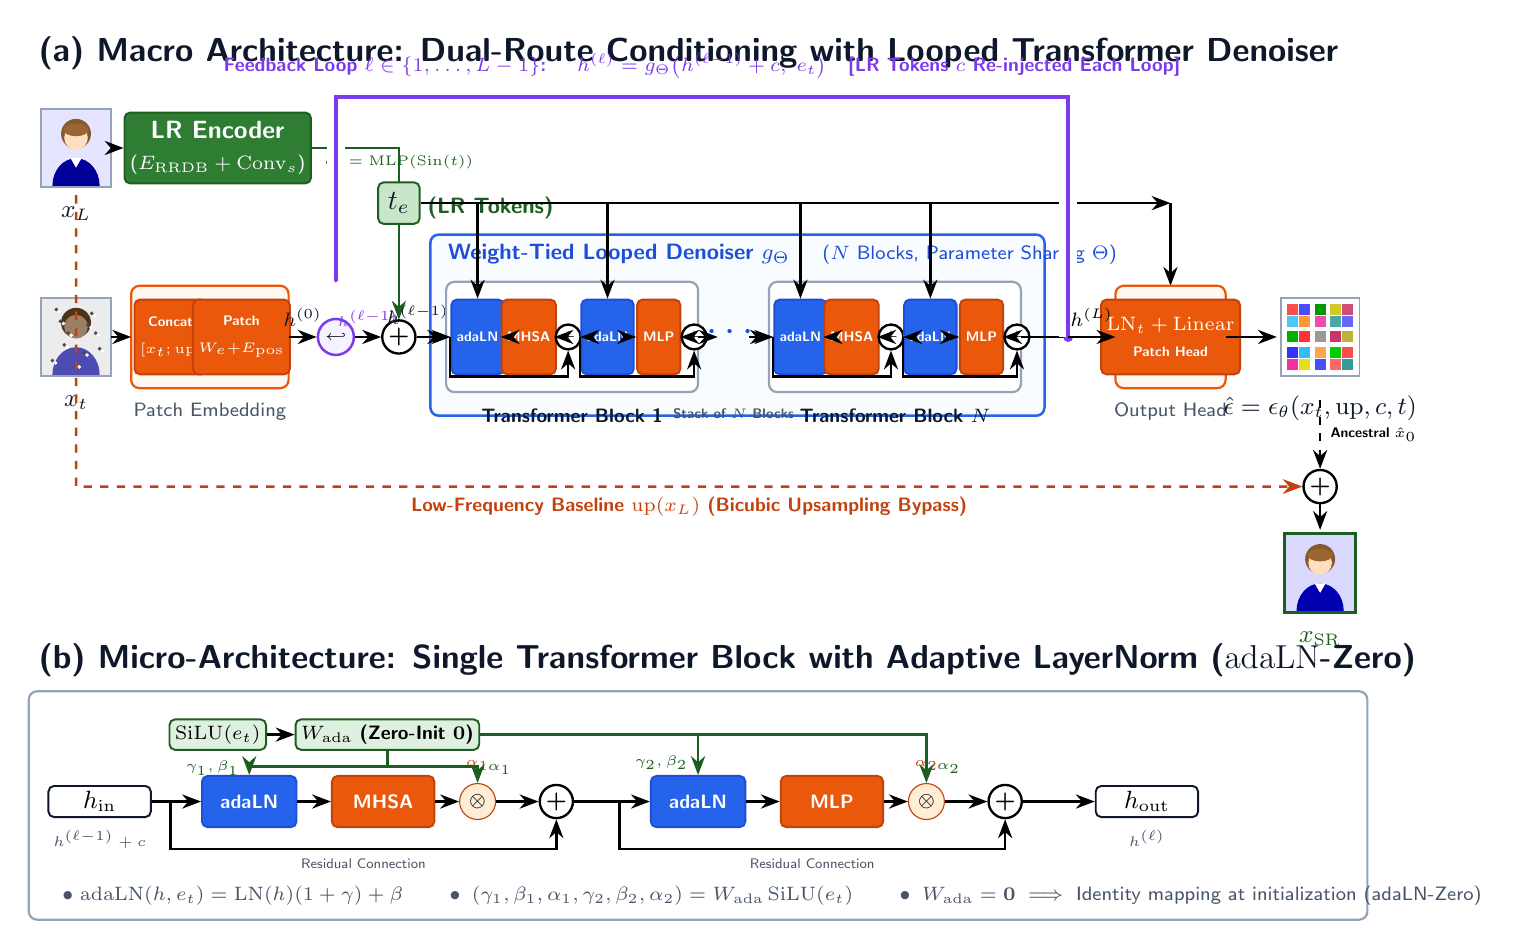
\begin{tikzpicture}[
  >=Stealth,
  font=\small,
  node distance=0.5cm,
  % Node Styles
  srdiffBase/.style={
    draw=BorderGray,
    line width=0.7pt,
    rounded corners=2pt,
    align=center,
    inner sep=2pt
  },
  srdiffContainer/.style={
    draw=BorderGray,
    line width=0.8pt,
    rounded corners=3pt,
    fill=ContainerGray
  },
  srdiffStripOrange/.style={
    srdiffBase,
    fill=SRPeachMid,
    draw=SRPeachDark,
    text=white,
    font=\footnotesize\bfseries
  },
  srdiffStripBlue/.style={
    srdiffBase,
    fill=SRBlueMid,
    draw=SRBlueDark,
    text=white,
    font=\footnotesize\bfseries
  },
  srdiffStripGreen/.style={
    srdiffBase,
    fill=SRGreenMid,
    draw=SRGreenDark,
    text=white,
    font=\footnotesize\bfseries
  },
  plusCircle/.style={
    circle,
    draw=black,
    line width=0.85pt,
    fill=white,
    inner sep=0pt,
    minimum size=12pt,
    font=\footnotesize\bfseries
  },
  busArrow/.style={
    ->,
    line width=0.85pt,
    draw=black
  },
  loopArrow/.style={
    ->,
    line width=1.3pt,
    draw=SRLoopPurple
  }
]

  % =========================================================================
  % SUBFIGURE (A): MACRO ARCHITECTURE PIPELINE
  % =========================================================================
  \begin{scope}[local bounding box=macroPipeline]
    
    % Subfigure Header
    \node[anchor=west, font=\large\bfseries, text=SlateText] at (0, 3.6) 
      {(a) Macro Architecture: Dual-Route Conditioning with Looped Transformer Denoiser};

    % -----------------------------------------------------------------------
    % Top Lane: LR Input x_L & LR Encoder
    % -----------------------------------------------------------------------
    \begin{scope}[shift={(0.6, 2.4)}]
      \draw[draw=BorderGray, fill=white, line width=0.7pt] (-0.45, -0.5) rectangle (0.45, 0.5);
      \fill[blue!10] (-0.43, -0.48) rectangle (0.43, 0.48);
      % Portrait avatar
      \fill[brown!70!black] (0, 0.18) circle (0.19);
      \fill[orange!25!white] (0, 0.13) circle (0.15);
      \fill[brown!80!black] (0, 0.23) ellipse (0.16 and 0.08);
      \fill[blue!60!black] (-0.3, -0.48) arc (180:0:0.3 and 0.35) -- cycle;
      \fill[white] (-0.07, -0.13) -- (0.07, -0.13) -- (0, -0.25) -- cycle;
    \end{scope}
    \node[below=2pt, font=\small\bfseries, text=SlateText] at (0.6, 1.85) {$x_L$};

    % LR Encoder Box
    \node[srdiffBase, fill=SRGreenMid, draw=SRGreenDark, text=white, minimum width=2.2cm, minimum height=0.9cm] 
      (lrEnc) at (2.4, 2.4) {\textbf{LR Encoder} \\ \scriptsize ($E_{\mathrm{RRDB}} + \mathrm{Conv}_s$)};

    \draw[busArrow] (1.05, 2.4) -- (lrEnc.west);

    % LR conditioning route into adder
    \draw[busArrow, draw=SRGreenDark] (lrEnc.east) -- (4.7, 2.4) 
      -- node[pos=0.35, right, font=\footnotesize\bfseries, text=SRGreenDark] {$c$ (LR Tokens)} 
      (4.7, 0.22);

    % -----------------------------------------------------------------------
    % Bottom Lane: Noisy Residual x_t & Initial Patch Embedding
    % -----------------------------------------------------------------------
    \begin{scope}[shift={(0.6, 0.0)}]
      \draw[draw=BorderGray, fill=white, line width=0.7pt] (-0.45, -0.5) rectangle (0.45, 0.5);
      \fill[gray!15] (-0.43, -0.48) rectangle (0.43, 0.48);
      % Face silhouette
      \fill[brown!40!black] (0, 0.18) circle (0.19);
      \fill[orange!20!gray] (0, 0.13) circle (0.15);
      \fill[blue!40!gray] (-0.3, -0.48) arc (180:0:0.3 and 0.35) -- cycle;
      % Noise speckles
      \foreach \dx/\dy in {-0.3/-0.3, -0.2/0.2, 0.1/-0.2, 0.2/0.3, -0.1/0.05, 0.15/0.15, -0.15/-0.1, 0.3/-0.15, -0.25/0.35, 0.0/-0.35, 0.25/0.05} {
        \fill[black!70] (\dx, \dy) circle (0.025);
        \fill[white!90] (\dx+0.04, \dy-0.03) circle (0.025);
      }
    \end{scope}
    \node[below=2pt, font=\small\bfseries, text=SlateText] at (0.6, -0.55) {$x_t$};

    % Patch Embedding Container
    \draw[srdiffContainer, fill=SRPeachLight!40, draw=SRPeachMid] (1.3, -0.65) rectangle (3.3, 0.65);
    \node[srdiffStripOrange, minimum width=0.7cm, minimum height=0.95cm] at (1.8, 0.0) 
      {\tiny Concat \\ \tiny $[x_t ; \mathrm{up}]$};
    \node[srdiffStripOrange, minimum width=0.7cm, minimum height=0.95cm] at (2.7, 0.0) 
      {\tiny Patch \\ \tiny $W_e {+} E_{\mathrm{pos}}$};
    \node[below=1pt, font=\scriptsize, text=SubText] at (2.3, -0.68) {Patch Embedding};

    \draw[busArrow] (1.05, 0.0) -- (1.3, 0.0);

    % Loop Multiplexer / Recurrent State Junction
    \node[circle, draw=SRLoopPurple, fill=SRLoopBg, line width=0.9pt, inner sep=0pt, minimum size=13pt] 
      (loopMux) at (3.9, 0.0) {\tiny $\hookleftarrow$};
    \draw[busArrow] (3.3, 0.0) -- (loopMux.west) 
      node[midway, above, font=\scriptsize\bfseries, text=SlateText] {$h^{(0)}$};

    % Re-Injection Adder Circle: h^{(\ell-1)} + c
    \node[plusCircle] (cAdder) at (4.7, 0.0) {$\boldsymbol{+}$};
    \draw[busArrow] (loopMux.east) -- (cAdder.west) 
      node[midway, above, font=\tiny\bfseries, text=SRLoopPurple] {$h^{(\ell-1)}$};

    % -----------------------------------------------------------------------
    % Timestep Indicator t_e
    % -----------------------------------------------------------------------
    \node[srdiffBase, fill=SRGreenLight, draw=SRGreenDark, text=SlateText, font=\bfseries, minimum size=15pt] 
      (teBox) at (4.7, 1.7) {$t_e$};
    \node[above=1pt of teBox, font=\tiny\bfseries, text=SRGreenDark] {$e_t = \mathrm{MLP}(\mathrm{Sin}(t))$};

    % -----------------------------------------------------------------------
    % Middle Part: Looped Transformer Denoiser Stack g_Theta
    % -----------------------------------------------------------------------
    \draw[srdiffContainer, fill=SRBlueBg!35, draw=SRBlueMid, line width=0.9pt] 
      (5.1, -1.0) rectangle (12.9, 1.3);
    
    \node[anchor=west, font=\footnotesize\bfseries, text=SRBlueDark] at (5.2, 1.05) 
      {Weight-Tied Looped Denoiser $g_\Theta$ \quad \normalfont\scriptsize ($N$ Blocks, Parameter Sharing $\Theta$)};

    \draw[busArrow] (cAdder.east) -- (5.3, 0.0) 
      node[midway, above, font=\scriptsize\bfseries, text=SlateText] {$h^{(\ell-1)} {+} c$};

    % --- Transformer Block 1 ---
    \draw[srdiffContainer, fill=white, draw=BorderGray] (5.3, -0.7) rectangle (8.5, 0.7);
    \node[srdiffStripBlue, minimum width=0.45cm, minimum height=0.95cm] (b1_ln1) at (5.7, 0.0) {\tiny adaLN};
    \node[srdiffStripOrange, minimum width=0.55cm, minimum height=0.95cm] (b1_mhsa) at (6.35, 0.0) {\tiny MHSA};
    \node[plusCircle, minimum size=9pt] (b1_add1) at (6.85, 0.0) {\tiny $+$};
    \node[srdiffStripBlue, minimum width=0.45cm, minimum height=0.95cm] (b1_ln2) at (7.35, 0.0) {\tiny adaLN};
    \node[srdiffStripOrange, minimum width=0.55cm, minimum height=0.95cm] (b1_mlp) at (8.0, 0.0) {\tiny MLP};
    \node[plusCircle, minimum size=9pt] (b1_add2) at (8.45, 0.0) {\tiny $+$};
    
    % Block 1 internal flow and residual lines
    \draw[busArrow] (5.3, 0.0) -- (b1_ln1.west);
    \draw[busArrow] (b1_ln1) -- (b1_mhsa);
    \draw[busArrow] (b1_mhsa) -- (b1_add1);
    \draw[busArrow] (b1_add1) -- (b1_ln2);
    \draw[busArrow] (b1_ln2) -- (b1_mlp);
    \draw[busArrow] (b1_mlp) -- (b1_add2);
    \draw[busArrow] (5.35, 0.0) -- ++(0, -0.5) -| (b1_add1.south);
    \draw[busArrow] (7.0, 0.0) -- ++(0, -0.5) -| (b1_add2.south);
    
    \node[below=2pt, font=\scriptsize\bfseries, text=SlateText] at (6.9, -0.72) {Transformer Block 1};

    % --- Inter-block connection & Ellipsis ---
    \draw[busArrow] (8.5, 0.0) -- (8.75, 0.0);
    \node[font=\Large\bfseries, text=SRBlueDark] at (8.95, 0.05) {$\cdots$};
    \node[below=2pt, font=\tiny\bfseries, text=SubText] at (8.95, -0.72) {Stack of $N$ Blocks};
    \draw[busArrow] (9.15, 0.0) -- (9.4, 0.0);

    % --- Transformer Block N ---
    \draw[srdiffContainer, fill=white, draw=BorderGray] (9.4, -0.7) rectangle (12.6, 0.7);
    \node[srdiffStripBlue, minimum width=0.45cm, minimum height=0.95cm] (bn_ln1) at (9.8, 0.0) {\tiny adaLN};
    \node[srdiffStripOrange, minimum width=0.55cm, minimum height=0.95cm] (bn_mhsa) at (10.45, 0.0) {\tiny MHSA};
    \node[plusCircle, minimum size=9pt] (bn_add1) at (10.95, 0.0) {\tiny $+$};
    \node[srdiffStripBlue, minimum width=0.45cm, minimum height=0.95cm] (bn_ln2) at (11.45, 0.0) {\tiny adaLN};
    \node[srdiffStripOrange, minimum width=0.55cm, minimum height=0.95cm] (bn_mlp) at (12.1, 0.0) {\tiny MLP};
    \node[plusCircle, minimum size=9pt] (bn_add2) at (12.55, 0.0) {\tiny $+$};
    
    % Block N internal flow and residual lines
    \draw[busArrow] (9.4, 0.0) -- (bn_ln1.west);
    \draw[busArrow] (bn_ln1) -- (bn_mhsa);
    \draw[busArrow] (bn_mhsa) -- (bn_add1);
    \draw[busArrow] (bn_add1) -- (bn_ln2);
    \draw[busArrow] (bn_ln2) -- (bn_mlp);
    \draw[busArrow] (bn_mlp) -- (bn_add2);
    \draw[busArrow] (9.45, 0.0) -- ++(0, -0.5) -| (bn_add1.south);
    \draw[busArrow] (11.1, 0.0) -- ++(0, -0.5) -| (bn_add2.south);
    
    \node[below=2pt, font=\scriptsize\bfseries, text=SlateText] at (11.0, -0.72) {Transformer Block $N$};

    % Timestep Distribution Bus
    \draw[busArrow] (teBox.east) -- (14.5, 1.7);
    \draw[busArrow] (5.7, 1.7) -- (b1_ln1.north);
    \draw[busArrow] (7.35, 1.7) -- (b1_ln2.north);
    \draw[busArrow] (9.8, 1.7) -- (bn_ln1.north);
    \draw[busArrow] (11.45, 1.7) -- (bn_ln2.north);
    \draw[busArrow] (14.5, 1.7) -- (14.5, 0.65);

    % Block Output to Junction Node
    \coordinate (junction) at (13.2, 0.0);
    \draw[line width=0.85pt] (12.6, 0.0) -- (junction);
    \fill[SRLoopPurple] (junction) circle (1.8pt);

    % -----------------------------------------------------------------------
    % The Recurrent Feedback Loop
    % -----------------------------------------------------------------------
    \draw[loopArrow, double=SRLoopPurple, double distance=1.3pt, draw=white, line width=2.7pt] 
      (junction) -- (13.2, 3.05) 
      -- node[above=2pt, font=\scriptsize\bfseries, text=SRLoopPurple] 
         {Feedback Loop $\ell \in \{1,\dots,L-1\}$: \quad $h^{(\ell)} = g_\Theta\big(h^{(\ell-1)} + c,\; e_t\big) \quad \text{[LR Tokens $c$ Re-injected Each Loop]}$}
         (3.9, 3.05) 
      -- (loopMux.north);

    % -----------------------------------------------------------------------
    % Output Head & Noise Map Thumbnail \hat{\epsilon}
    % -----------------------------------------------------------------------
    \draw[srdiffContainer, fill=SRPeachLight!40, draw=SRPeachMid] (13.8, -0.65) rectangle (15.2, 0.65);
    \node[srdiffStripOrange, minimum width=1.1cm, minimum height=0.95cm] (outHead) at (14.5, 0.0) 
      {\scriptsize $\mathrm{LN}_t + \mathrm{Linear}$ \\ \tiny Patch Head};
    \node[below=1pt, font=\scriptsize, text=SubText] at (14.5, -0.68) {Output Head};

    \draw[busArrow] (junction) -- (13.8, 0.0) 
      node[midway, above, font=\scriptsize\bfseries] {$h^{(L)}$};

    % Output Noise Map Thumbnail \hat{\epsilon}
    \begin{scope}[shift={(16.4, 0.0)}]
      \draw[draw=BorderGray, fill=white, line width=0.7pt] (-0.5, -0.5) rectangle (0.5, 0.5);
      % Multicolored RGB noise grid
      \foreach \x/\y/\col in {
        -0.35/0.35/red!70, -0.2/0.35/blue!70, 0.0/0.35/green!60!black, 0.2/0.35/yellow!80!black, 0.35/0.35/purple!70,
        -0.35/0.2/cyan!70, -0.2/0.2/orange!80, 0.0/0.2/magenta!70, 0.2/0.2/teal!70, 0.35/0.2/blue!60,
        -0.35/0.0/green!70!black, -0.2/0.0/red!80, 0.0/0.0/gray!80, 0.2/0.0/purple!80, 0.35/0.0/yellow!70!black,
        -0.35/-0.2/blue!80, -0.2/-0.2/cyan!80, 0.0/-0.2/orange!70, 0.2/-0.2/green!80!black, 0.35/-0.2/red!70,
        -0.35/-0.35/magenta!80, -0.2/-0.35/yellow!90!black, 0.0/-0.35/blue!70, 0.2/-0.35/red!60, 0.35/-0.35/teal!80
      } {
        \fill[\col] (\x-0.07, \y-0.07) rectangle (\x+0.07, \y+0.07);
      }
    \end{scope}
    \node[below=2pt, font=\small\bfseries, text=SlateText] at (16.4, -0.55) {$\hat{\epsilon} = \epsilon_\theta(x_t, \mathrm{up}, c, t)$};

    \draw[busArrow] (15.2, 0.0) -- (15.85, 0.0);

    % -----------------------------------------------------------------------
    % Low-Frequency Residual Addition & Reconstruction
    % -----------------------------------------------------------------------
    \node[plusCircle] (reconAdd) at (16.4, -1.9) {$\boldsymbol{+}$};
    \draw[busArrow, dashed] (16.4, -0.8) -- (reconAdd.north) 
      node[midway, right, font=\tiny\bfseries] {Ancestral $\hat{x}_0$};

    % SR Output Thumbnail
    \begin{scope}[shift={(16.4, -3.0)}]
      \draw[draw=SRGreenDark, fill=white, line width=1.0pt] (-0.45, -0.5) rectangle (0.45, 0.5);
      \fill[blue!15] (-0.43, -0.48) rectangle (0.43, 0.48);
      % High resolution face avatar
      \fill[brown!70!black] (0, 0.18) circle (0.19);
      \fill[orange!25!white] (0, 0.13) circle (0.15);
      \fill[brown!80!black] (0, 0.23) ellipse (0.16 and 0.08);
      \fill[blue!70!black] (-0.3, -0.48) arc (180:0:0.3 and 0.35) -- cycle;
      \fill[white] (-0.07, -0.13) -- (0.07, -0.13) -- (0, -0.25) -- cycle;
    \end{scope}
    \node[below=2pt, font=\small\bfseries, text=SRGreenDark] at (16.4, -3.55) {$x_{\mathrm{SR}}$};
    \draw[busArrow] (reconAdd.south) -- (16.4, -2.45);

    % Bicubic baseline running from input x_L to reconstruction adder
    \draw[busArrow, draw=SRPeachDark, dashed, line width=0.9pt] 
      (0.6, 1.8) -- ++(0, -3.7) 
      -- node[below, font=\scriptsize\bfseries, text=SRPeachDark] 
         {Low-Frequency Baseline $\mathrm{up}(x_L)$ (Bicubic Upsampling Bypass)} 
         (reconAdd.west);

  \end{scope}

  % =========================================================================
  % SUBFIGURE (B): TRANSFORMER BLOCK MICRO-ARCHITECTURE WITH adaLN-ZERO
  % =========================================================================
  \begin{scope}[shift={(0, -5.8)}, local bounding box=microBlock]
    
    % Subfigure Header
    \node[anchor=west, font=\large\bfseries, text=SlateText] at (0, 1.7) 
      {(b) Micro-Architecture: Single Transformer Block with Adaptive LayerNorm ($\mathrm{adaLN}$-Zero)};

    % Micro Outer Frame
    \draw[srdiffContainer, fill=white, draw=BorderGray, line width=0.8pt] 
      (0, -1.6) rectangle (17.0, 1.3);

    % Block Input Token
    \node[srdiffBase, fill=white, draw=SlateText, font=\small\bfseries, minimum width=1.3cm] 
      (hin) at (0.9, -0.1) {$h_{\mathrm{in}}$};
    \node[below=1pt of hin, font=\tiny, text=SubText] {$h^{(\ell-1)} + c$};

    % Timestep Modulator Engine (adaLN parameter generator)
    \node[srdiffBase, fill=SRGreenLight!60, draw=SRGreenDark, font=\scriptsize\bfseries] 
      (silu) at (2.4, 0.75) {$\mathrm{SiLU}(e_t)$};
    \node[srdiffBase, fill=SRGreenLight!60, draw=SRGreenDark, font=\scriptsize\bfseries, right=0.35cm of silu] 
      (wada) {$W_{\mathrm{ada}}$ (Zero-Init $\mathbf{0}$)};
    \draw[busArrow] (silu) -- (wada);

    % Sub-Layer 1: Self-Attention (MHSA)
    \coordinate (split1) at (1.8, -0.1);
    \node[srdiffStripBlue, minimum width=1.2cm, minimum height=0.65cm] (mb_ln1) at (2.8, -0.1) {\scriptsize adaLN};
    \node[srdiffStripOrange, minimum width=1.3cm, minimum height=0.65cm] (mb_mhsa) at (4.5, -0.1) {\scriptsize MHSA};
    
    \node[circle, draw=SRPeachDark, fill=SRPeachLight, inner sep=0pt, minimum size=13pt, font=\scriptsize\bfseries] 
      (gate1) at (5.7, -0.1) {$\otimes$};
    \node[above=1pt of gate1, font=\tiny\bfseries, text=SRPeachDark] {$\alpha_1$};

    \node[plusCircle] (mb_add1) at (6.7, -0.1) {$\boldsymbol{+}$};

    % Sub-Layer 2: Feed-Forward Network (MLP)
    \coordinate (split2) at (7.5, -0.1);
    \node[srdiffStripBlue, minimum width=1.2cm, minimum height=0.65cm] (mb_ln2) at (8.5, -0.1) {\scriptsize adaLN};
    \node[srdiffStripOrange, minimum width=1.3cm, minimum height=0.65cm] (mb_mlp) at (10.2, -0.1) {\scriptsize MLP};

    \node[circle, draw=SRPeachDark, fill=SRPeachLight, inner sep=0pt, minimum size=13pt, font=\scriptsize\bfseries] 
      (gate2) at (11.4, -0.1) {$\otimes$};
    \node[above=1pt of gate2, font=\tiny\bfseries, text=SRPeachDark] {$\alpha_2$};

    \node[plusCircle] (mb_add2) at (12.4, -0.1) {$\boldsymbol{+}$};

    % Block Output Token
    \node[srdiffBase, fill=white, draw=SlateText, font=\small\bfseries, minimum width=1.3cm] 
      (hout) at (14.2, -0.1) {$h_{\mathrm{out}}$};
    \node[below=1pt of hout, font=\tiny, text=SubText] {$h^{(\ell)}$};

    % Flow connections
    \draw[busArrow] (hin) -- (mb_ln1);
    \draw[busArrow] (mb_ln1) -- (mb_mhsa);
    \draw[busArrow] (mb_mhsa) -- (gate1);
    \draw[busArrow] (gate1) -- (mb_add1);
    \draw[busArrow] (mb_add1) -- (mb_ln2);
    \draw[busArrow] (mb_ln2) -- (mb_mlp);
    \draw[busArrow] (mb_mlp) -- (gate2);
    \draw[busArrow] (gate2) -- (mb_add2);
    \draw[busArrow] (mb_add2) -- (hout);

    % Residual connections
    \draw[busArrow] (split1) -- ++(0, -0.6) -| (mb_add1.south) 
      node[pos=0.25, below, font=\tiny, text=SubText] {Residual Connection};
    \draw[busArrow] (split2) -- ++(0, -0.6) -| (mb_add2.south) 
      node[pos=0.25, below, font=\tiny, text=SubText] {Residual Connection};

    % Modulation arrows from W_ada (Clean non-overlapping distribution)
    \draw[busArrow, draw=SRGreenDark] (wada.south) -- ++(0, -0.2) -| (mb_ln1.north) 
      node[pos=0.6, left, font=\tiny\bfseries, text=SRGreenDark] {$\gamma_1, \beta_1$};
    \draw[busArrow, draw=SRGreenDark] (wada.south) -- ++(0, -0.2) -| (gate1.north)
      node[pos=0.6, right, font=\tiny\bfseries, text=SRGreenDark] {$\alpha_1$};
    \draw[busArrow, draw=SRGreenDark] (wada.east) -- (8.5, 0.75) -- (mb_ln2.north) 
      node[pos=0.7, left, font=\tiny\bfseries, text=SRGreenDark] {$\gamma_2, \beta_2$};
    \draw[busArrow, draw=SRGreenDark] (8.5, 0.75) -- (11.4, 0.75) -- (gate2.north)
      node[pos=0.7, right, font=\tiny\bfseries, text=SRGreenDark] {$\alpha_2$};

    % Math Callout Summary
    \node[anchor=west, font=\scriptsize, text=SubText] at (0.3, -1.3) 
      {$\bullet\;\mathrm{adaLN}(h, e_t) = \mathrm{LN}(h)(1+\gamma) + \beta \qquad \bullet\;(\gamma_1, \beta_1, \alpha_1, \gamma_2, \beta_2, \alpha_2) = W_{\mathrm{ada}}\,\mathrm{SiLU}(e_t) \qquad \bullet\;W_{\mathrm{ada}}=\mathbf{0} \implies \text{Identity mapping at initialization (adaLN-Zero)}$};

  \end{scope}

\end{tikzpicture}
\end{center}

\vspace{-0.3cm}
\captionof{figure}{\textbf{Overview of the Proposed Looped Diffusion Transformer Architecture (derived from the SRDiff pipeline).} 
\textbf{(a) Macro Pipeline:} Following the residual diffusion framework, low-frequency content is carried directly by the bicubic upsampled input $\mathrm{up}(x_L)$, leaving the diffusion model to synthesize only the missing high-frequency residual $x_0 = x_H - \mathrm{up}(x_L)$. Conditioning is performed via two synchronized routes: (i) spatial concatenation $[\,x_t \,;\, \mathrm{up}(x_L)\,]$ linearly projected into initial tokens $h^{(0)}$, and (ii) an RRDB convolutional encoder with strided convolution yielding aligned tokens $c$. In place of the multi-scale convolutional U-Net denoiser, our model introduces a weight-tied looped transformer stack $g_\Theta$ containing $N$ blocks. Over $L$ loop iterations, the LR representation $c$ is explicitly re-injected ($h^{(\ell-1)} + c$), achieving an effective depth of $N \times L$ with only $N$ parameter blocks. The output head maps tokens $h^{(L)}$ to the predicted noise $\hat{\epsilon}$, from which $\hat{x}_0$ is sampled and summed with $\mathrm{up}(x_L)$ to produce $x_{\mathrm{SR}}$. 
\textbf{(b) Micro-Architecture:} Single transformer block with adaptive LayerNorm ($\mathrm{adaLN}$-Zero), showing scale/shift modulation $(\gamma, \beta)$ and residual gating factors $\alpha_1, \alpha_2$ governed by zero-initialized $W_{\mathrm{ada}}$.}
\label{fig:looped_diff_transformer}

\end{document}